%% ****** Start of file apsguide4-2.tex ****** %
%%
%%   This file is part of the APS files in the REVTeX 4.2 distribution.
%%   Version 4.2b of REVTeX, December 2018.
%%
%%   Copyright (c) 2019 The American Physical Society.
%%
%%   See the REVTeX 4.2 README file for restrictions and more information.
%%
\documentclass[twocolumn, nofootinbib, secnumarabic, amssymb, nobibnotes, aps, prd]{revtex4-2}
\usepackage{graphicx}
%\usepackage{acrofont}%NOTE: Comment out this line for the release version!
\newcommand{\revtex}{REV\TeX\ }
\newcommand{\classoption}[1]{\texttt{#1}}
\newcommand{\macro}[1]{\texttt{\textbackslash#1}}
\newcommand{\m}[1]{\macro{#1}}
\newcommand{\env}[1]{\texttt{#1}}
\setlength{\textheight}{9.5in}

\begin{document}

\title{Predicting Superconducting Critical Temperatures with Supervised Machine Learning\thanks{Work supported by the National Science Foundation}}

\author{K. Kleinasser, Cornell University, Ithaca, NY}
\altaffiliation{Lycoming College, Williamsport, PA}
\email{klekirk@lycoming.edu}

\maketitle
\tableofcontents

\section{Introduction}
\subsection{Superconductors}
Superconductors are materials that lose all electrical resistance at low temperatures. These materials have a critical temperature ($T_C$) at which they lose their resistance. Most have very low critical temperatures, but “unconventional superconductors” can have critical temperatures as high as room temperature under non-atmospheric conditions. 

Electrons in superconductors form Cooper Pairs below their critical temperature. These pairs of electrons are held together with phonouns, which are atomic-level collective excitations. Phonouns are similar to photons in that they also have particle-like properties \cite{rohlf_1994}.

Unconventional superconductors are still not well understood and remain an open question in Physics. Understanding them could lead to the discovery of superconducting materials stable at room temperature under atmospheric conditions. Such a material would have large implications, such as super efficient electricity transfer and vast efficiency improvements for applications like particle accelerators and power lines.


\subsection{Matminer}
Most superconducter databases do not include enough information to train an effective machine learning model, but such data can be extracted from the data they do provide. We use matminer to produce our features from the provided material data. Matminer is a python library that generates data from various measured properties of a material. Matminer collects existing calculations into a machine learning friendly python package. Our matminer workflow is shown in Figure~\ref{fig:matminer-flowchart}.

\begin{figure}[!htb]
   \centering
   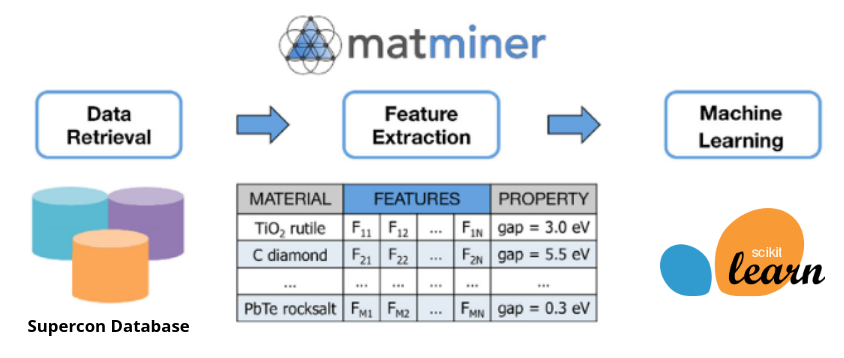
\includegraphics[scale=0.25]{flowchart.png}
   \caption{Flowchart illustrating our matminer usage, modified from official matminer graphic \cite{WARD201860}.}
   \label{fig:matminer-flowchart}
\end{figure}

Our database only provides the superconductor composition data. Matminer's featurizers can generate 53 features from the composition of a material. If we had band structure or other data, we could produce more information that we could use in our model.

\subsection{Machine Learning}
Previous papers have used random forest models to predict critical temperature [citation needed], but this paper will examine eight models before settling on two for further investigation. These models are described below. Each model's hyperparameters\footnote{Hyperparameters are machine learning parameters that change how a model is trained.} was optimized with Scikit-Learn's GridSearchCV, which tests combinations from a grid of hyperparameters and returns the best performing model based on a specified metric. 

We started our model search with some linear models. Besides the base Linear Regression model, we used linear (and polynomial) Support Vector Regression (SVR) models. SVR uses decision boundaries, which are lines parallel to the regression line. The model aims to maximize the amount of data within the decision boundaries and has hyperparamters to modify sensitivity to prevent overfitting.\footnote{Overfitting occurs when a model is trained to be too specific to a particular dataset and is not generalizable.} We also trialed Elastic Net and Bayesian Ridge models. Elastic Net uses L1 and L2 penalties to stabilize the model, and Bayesian Ridge uses probability distributors instead of point estimates.

Additionally, we trialed Decision Tree and KNeighbors (KNN) models. Decision trees are very interpretable - they break predictions into nodes of the tree, eventually leading to a prediction value. These trees can be represented graphically and show how they produce results, unlike most machine learning models. KNN models are a little different, they store all the data and predict values based on a similarity measure. The model looks at a specified number of similar neighbors to produce a prediction.

Finally, we tried multiple ensemble models - Random Forest Regression (RFR), Extra Trees, and a superlearner. RFR models use numerous decision trees and subsamples the data with replacement. This means that the model replace data after using it in a subset. Extra Trees is like RFR, but it does not replace the data after use in a subset. The final ensemble model we tested is a superlearner, a model that can combine multiple high-scoring Scikit-Learn model predictions and sometimes improve the performance from the individual models.


\section{Methodology}
\subsection{Code Structure}
The source code used for this paper is available publicly on github at \url{https://github.com/sylphrena0/classe2022}. This repository also includes the source files for this latex paper, data files, images, and documentation files.

The code is split into multiple python files so processes could be completed in stages and to maintain readability in the code. Most of our testing and final training was completed in juypter notebooks, but some computations were highly computationally expensive and needed to be run remotely. For these jobs, we created simple python files and made bash scripts to run them on Cornell's CLASSE compute farm. We also made several bash aliases and functions to simplify the compute farm workflow, which are also available on the github repository. 

Since we used multiple files, we chose to create shared dependencies files where we defined functions to import data, train models, and generate our graphs. These files are then imported in all the relevant scripts to reduce redundancy.

\subsection{Running the Code}

First, the featurizer script imports the dataset, extracts features from the material compositions, and exports the csv data. This script is one of the most computationally expensive and takes several hours to run on the CLASSE compute farm with 64 dedicated cores.

After the features are exported, our analysis jupyter notebook imports the data with the shared import function and exports histograms and a correlation matrix. 

Next, the training\_single jupyter notebook or script can train individual models with the shared evaluation functions. This is used to get a landscape of initial performance before optimization. After training, the function plots the actual $T_C$ versus the model prediction, using a heatmap to visualize the difference from the ideal prediction.

The optimizer script then uses a grid of manually defined hyperparameters to optimize models based on R2 score. This allowed significant improvements to baseline models. After optimization, the optimized models can be plotted in our single training notebook. After confirmation that the model is better than the baseline, the models can then be plotted together in a single graph using our bulk training notebook. 

We evaluated our models using several metrics - R2 scores for regression evaluation, Mean Squared Error (MSE) and Mean Absolute Error (MAE) for error evaluation, and prediction intervals for uncertainty evaluation.

\subsection{Uncertainty}
Our evaluation functions can produce error calculation using mapie, forestci, or lolopy. 

\section{Results}

\subsection{Fonts}
It is preferable to avoid the older \TeX\ and \LaTeX\ 2.09 macros for
controlling fonts such as \m{rm}, \m{it}, \textit{etc.} Rather, it is
better to use the macros introduced in \LaTeXe.  If the older font
commands are used (they really should be avoided!), be sure to use
curly braces to properly limit the extent of the font
change. \verb+{\bf ...}+ is the correct method.
Commands for controlling text and math font changes are summarized in
Table~\ref{tab:fonts}.



\bibliographystyle{apsrev4-2}
\bibliography{reu-report}
\end{document}

